\documentclass{beamer}
\usetheme[pageofpages=of,% String used between the current page and the
                         % total page count.
          bullet=circle,% Use circles instead of squares for bullets.
          titleline=true,% Show a line below the frame title.
          alternativetitlepage=true,% Use the fancy title page.
       %   titlepagelogo=logo-polito,% Logo for the first page.
       %   watermark=watermark-polito,% Watermark used in every page.
       %   watermarkheight=100px,% Height of the watermark.
       %   watermarkheightmult=4,% The watermark image is 4 times bigger
                                % than watermarkheight.
          ]{Torino}

\setbeamertemplate{footline}{
  \begin{beamercolorbox}[wd=\paperwidth,ht=1ex,dp=1ex]{footline}
    \vspace{5pt} \hspace{1em} \insertframenumber/\inserttotalframenumber
  \end{beamercolorbox}
}

\newcommand{\given}{\,|\,}

\usepackage{colortbl}
\definecolor{LightGray}{gray}{0.9}
\definecolor{DarkGray}{gray}{0.3}
\definecolor{LightCyan}{rgb}{0.9, 1, 1}
\definecolor{LightRed}{rgb}{1, 0.8, 0.8}
\definecolor{LightGreen}{rgb}{0.8, 1, 0.8}
\definecolor{DarkGreen}{rgb}{0.3, 0.5, 0.3}



\author{Brendon J. Brewer}
\title{Introduction to Bayesian Statistics}
\institute{Summer Institute in Statistical Genomics \\
The University of Auckland, November 2026}
\date{}


\linespread{1.3}
\usepackage{minted}
\usepackage[utf8]{inputenc}
\usepackage{dsfont}


\begin{document}

\frame{\titlepage}


\begin{frame}
\begin{center}
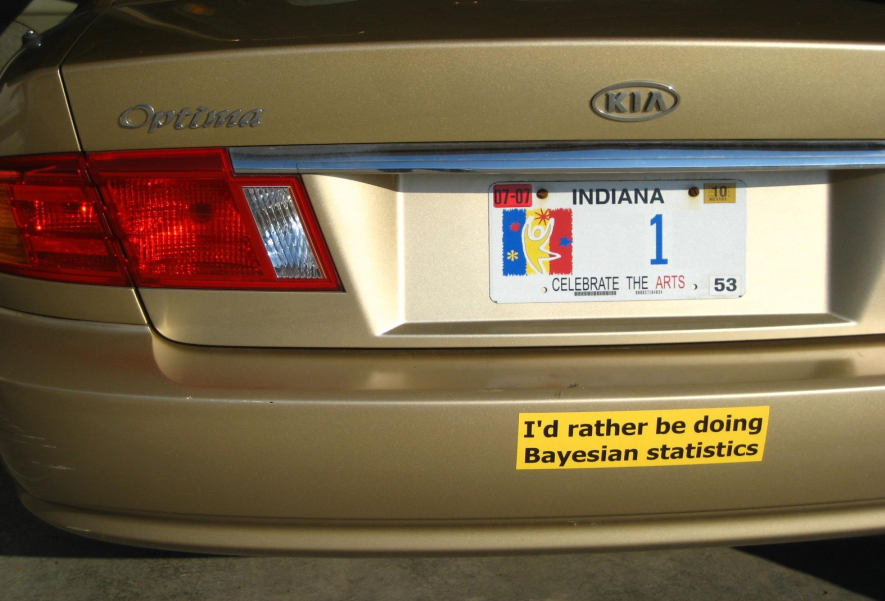
\includegraphics[width=0.6\textwidth]{images/bumper_sticker.png} \\
Credit: John Kruschke
\end{center}

\end{frame}




\begin{frame}
\frametitle{Parameter Estimation: Analytical Methods}

\begin{center}
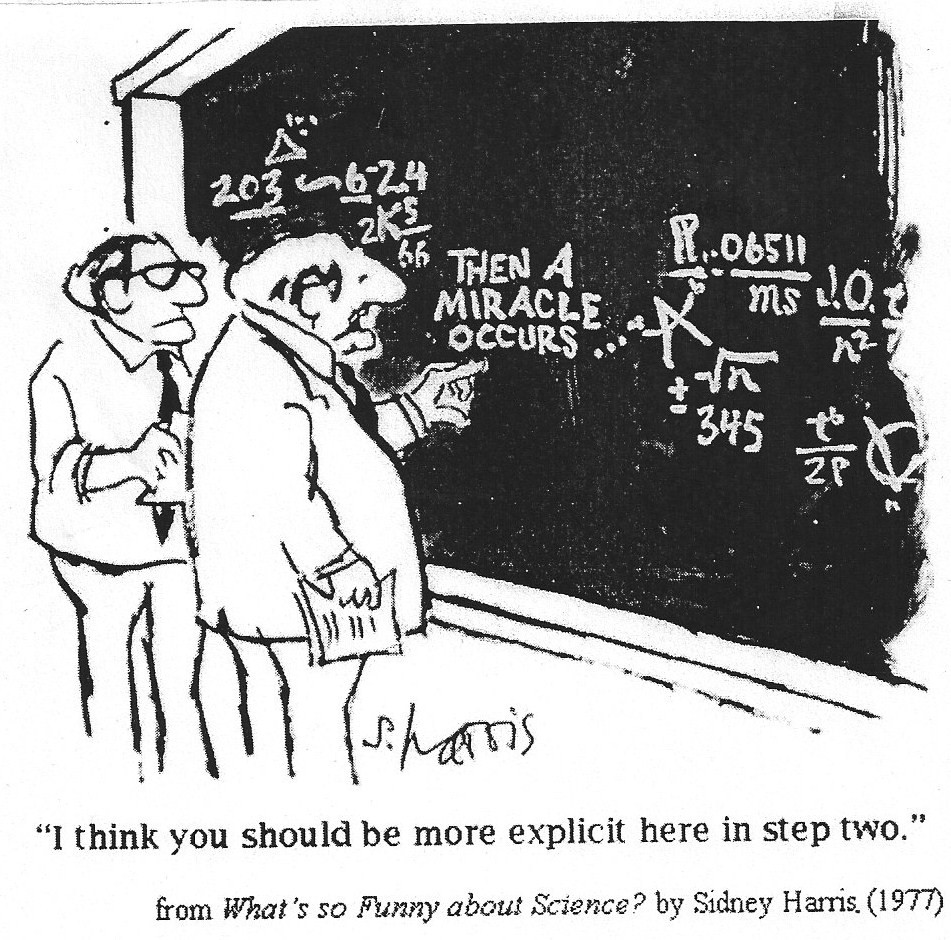
\includegraphics[width=0.6\textwidth]{images/miracle.jpg}
\end{center}

\end{frame}

\begin{frame}
\frametitle{Reminder of Bayes' Rule for Parameter Estimation}

\begin{align}
p(\theta \given x) &= \frac{p(\theta)p(x \given \theta)}{p(x)} \\
p(\theta \given x) &\propto p(\theta)p(x \given \theta) \\
\texttt{posterior} &\propto \texttt{prior} \times \texttt{likelihood}
\end{align}
(notation: $\theta$=parameter, $x$=data)\pause

In analytical methods, we will write down explicit mathematical expressions
for $p(\theta)$ and $p(x \given \theta)$, multiply them, and see what we
get for $p(\theta \given x)$.

\end{frame}


\begin{frame}
\frametitle{Reminder: Election Poll Problem}
We called 10 people and the data was
$\{1, 1, 0, 0, 1, 0, 1, 0, 1, 1\}$. Our likelihood function was
\begin{align}
p(x \given \theta) &= \theta^6(1-\theta)^4.
\end{align}
\pause
In this example, our parameter is actually called $\theta$ and our data may
as well be called $x$. In other problems, it's best to use the symbols
appropriate to the meanings of the parameter(s) and the data.
\end{frame}


\begin{frame}
\frametitle{Uniform Prior}
Let's choose a (continuous) uniform prior between 0 and 1 for $\theta$.
The mathematical expression for this density is
\begin{align}
p(\theta) = \left\{
                \begin{array}{cc}
                1, & 0 \leq \theta \leq 1 \\
                0, & \textnormal{otherwise}.
                \end{array}
            \right.
\end{align}
\pause
However, if we just remember that we're dealing with something between 0 and 1,
we can simply write
\begin{align}
p(\theta) = 1.
\end{align}

\end{frame}

\begin{frame}
\frametitle{Prior Times Likelihood}
By Bayes' rule, the posterior distribution is {\em proportional to}
the prior times the likelihood. We have those now:
\begin{align}
p(\theta \given x) &\propto p(\theta) p(x \given \theta) \\
                   &= 1 \times \theta^6(1-\theta)4 \\
                   &= \theta^6(1-\theta)^4.
\end{align}
\pause
We have the result! However, we need to understand what the distribution
looks like. We can (i) plot the function to see its shape (this will essentially
involve the Bayes Box steps!) or (ii) we can magically recognise from the
formula what this distribution must be.

\end{frame}


\begin{frame}
\frametitle{Beta Distributions}

\begin{itemize}
\item The {\bf beta distribution} is often used for values that are between 0
and 1.\pause
\item It has two parameters, $\alpha$ and $\beta$, which determine its shape.
For a quantity $x$ with a Beta distribution, we write $x \sim \textnormal{Beta}(\alpha, \beta)$.\pause
\item The probability density equation is
\begin{align}
p(x) &= \frac{1}{\textnormal{Beta}(\alpha, \beta)}
            x^{\alpha - 1}(1-x)^{\beta - 1}
\end{align} \pause
\item We mostly focus on the part that depends on $x$ - the other thing
at the front is just a normalisation constant.
\end{itemize}

\end{frame}

\begin{frame}
\frametitle{Comparing Formulas}

The beta distribution is
\begin{align}
p(x) &= \frac{1}{\textnormal{Beta}(\alpha, \beta)}
            x^{\alpha - 1}(1-x)^{\beta - 1}
\end{align}

and our posterior distribution was
\begin{align}
p(\theta \given x) &\propto \theta^6(1-\theta)^4.
\end{align}\pause
By comparing the two formulas, we see that our posterior is
a Beta$(7, 5)$ distribution. We can write
\begin{align}
\theta \given x &\sim \textnormal{Beta}(7, 5).
\end{align}

\end{frame}

\begin{frame}
\frametitle{Beta Distributions from Wikipedia}

\begin{center}
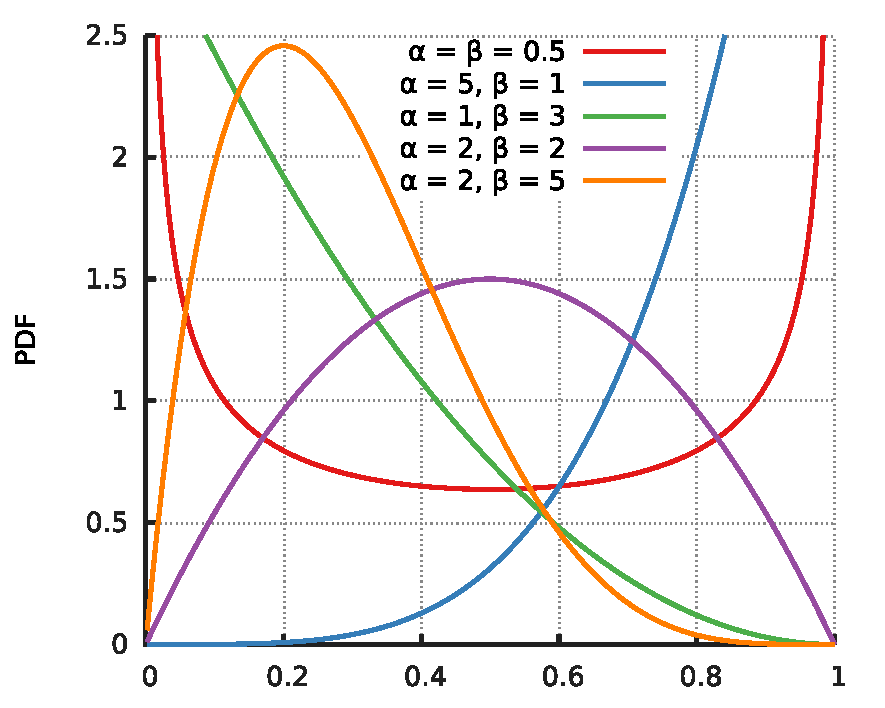
\includegraphics[width=0.6\textwidth]{images/betas.pdf}
\end{center}

\end{frame}

\begin{frame}
\frametitle{Our Beta(7, 5) Posterior}

\begin{center}
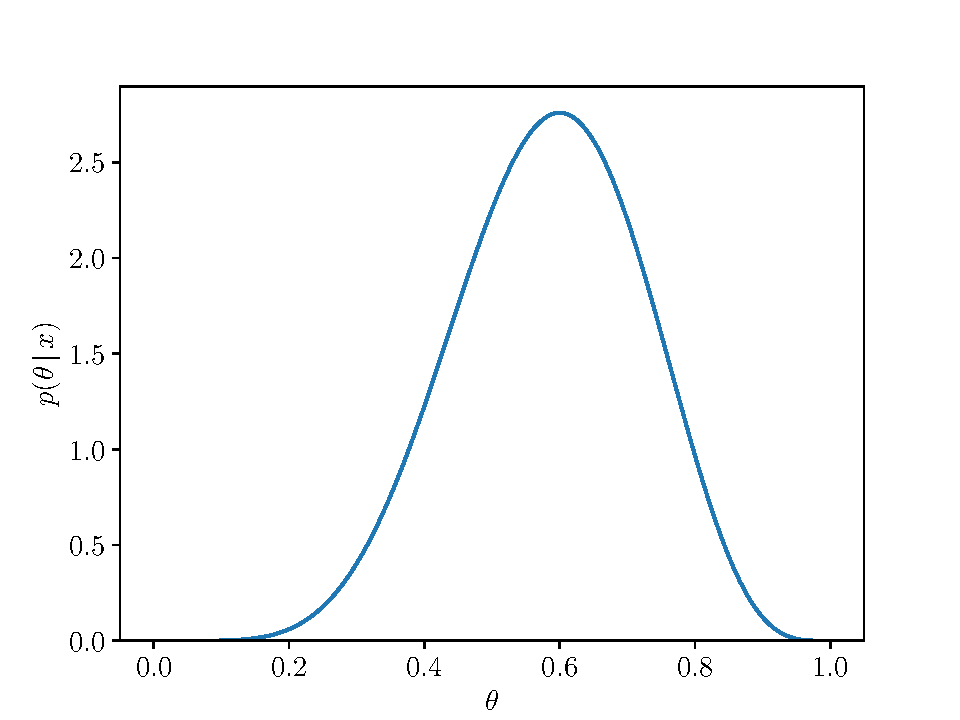
\includegraphics[width=0.6\textwidth]{images/beta_posterior.pdf}
\end{center}

\end{frame}

\begin{frame}
\frametitle{A Special Case}
The Beta(1, 1) distribution is actually the same as a Uniform(0, 1)
distribution. Look at the equation for the probability density:
\begin{align}
p(\theta) &\propto \theta^{\alpha-1}(1-\theta)^{\beta - 1} \\
          &= \theta^{0}(1-\theta)^{0} \\
          &= 1.
\end{align}

\end{frame}



\begin{frame}
\frametitle{Prediction}

\begin{itemize}
\item Let's do a Bayesian prediction using analytical methods. We will be
able to `cheat' instead of doing an integral.\pause
\item What is the probability that the `next' data point is a 1?\pause
\item This will give us Laplace's famous {\bf rule of succession}.
\end{itemize}

\end{frame}

\begin{frame}
\frametitle{Prediction: Bayesian Approach}

\begin{itemize}
\item Step 1: get the posterior distribution for the parameter(s)\pause
\item Step 2: For each possible value of the parameter, compute the probability
you're interested in (e.g., probability that the next data point is a 1).\pause
\item Step 3: Calculate the weighted average of the probabilities from the previous
step, using the posterior distribution for the weights.\pause
\end{itemize}

This procedure is not invented, but is derivable from the rules of
probability theory.

\end{frame}

\begin{frame}
\frametitle{Prediction: Bayesian Approach}
We've done step 1. For step two, consider: if we knew $\theta$, what would
be the probability of the next data point being a 1? Hopefully you can see that
it would simply be $\theta$ itself.\pause

Therefore to do the prediction we ``just'' need to do this integral:
\begin{align}
P(x_{11} = 1 \given x) &= \int_0^1 \theta p(\theta \given x)\, d\theta
\end{align}
where $p(\theta \given x)$ is our Beta$(7, 5)$ posterior. However, someone
has already done it for us!

\end{frame}

\begin{frame}
\frametitle{Expectation of a Beta Distribution}
You might recognise the previous integral as the definition of the
{\bf expectation} of our posterior distribution. Wikipedia has our answer.

\centering
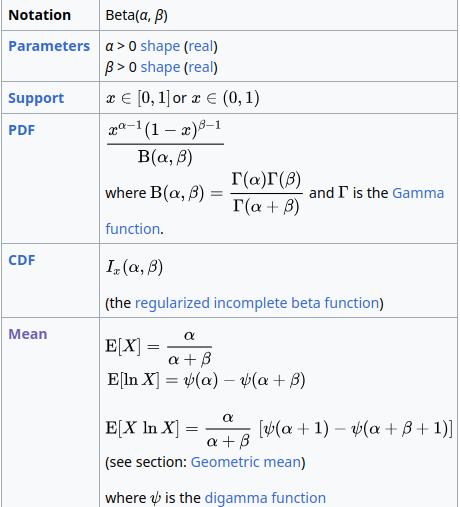
\includegraphics[scale=0.3]{images/wikipedia.png}

\end{frame}


\begin{frame}
\frametitle{Prediction Result}
Let's just use the given result.
\begin{align}
P(x_{11} = 1 \given x) &= \frac{7}{7+5} \\
                       &= 7/12.
\end{align}\pause
In general, for $x$ successes out of $N$ trials and a uniform prior for
$\theta$, the result is {\bf Laplace's rule of succession}:
\begin{align}
P(x_{\rm next} = 1 \given x) &= \frac{x+1}{N+2}.
\end{align}\pause
The result is {\em not} $x/N$, and continues to make sense even with no data
($x=N=0$)!


\end{frame}



\begin{frame}
\frametitle{Beta-Binomial}
Consider the binomial distribution, which is used for the number of successes
$x$ out of $N$ independent ``Bernoulli trials'', with success probability
$\theta$ on each of the trials. The Binomial distribution looks like
\begin{align}
p(x \given \theta) &= \binom{N}{x}\theta^x(1-\theta)^{N-x}.
\end{align}
\pause
If we observe the value of $x$ but want to infer $\theta$, we can derive
the posterior for $\theta$ given $x$. Let's do this now.

\end{frame}


\begin{frame}
\frametitle{Beta-Binomial}
There is a nice relationship between the beta distribution and the binomial
distribution. If the former is the prior for $\theta$ and the latter is the
sampling distribution (which gives the likelihood), then we get a nice
result.\pause
\begin{align}
p(\theta \given x) &\propto p(\theta) p(x \given \theta) \\
    &= \theta^{\alpha-1}(1-\theta)^{\beta-1} \theta^x(1-\theta)^{N-x} \\
    &= \theta^{\alpha+x-1}(1-\theta)^{\beta+N-x-1}
\end{align}
\pause
The posterior is another beta distribution!
\begin{align}
\theta \given x &\sim \textnormal{Beta}(\alpha+x, \beta+N-x)
\end{align}

\end{frame}

\begin{frame}
\frametitle{Rule of Succession}
If we take the expectation, like we did before, to find the predictive
probability of success on the next trial, we get
\begin{align}
\frac{\alpha+x}{\alpha + \beta + N}
\end{align}
as the result. If we choose a uniform prior ($\alpha=\beta=1$)
then we get the rule of succession again, which was
$(x+1)/(N+2)$.

\end{frame}



\begin{frame}
\frametitle{Conjugate Priors}
Beta Prior + Binomial Sampling Distribution $\implies$~
Beta Posterior \\

This is our first example of a {\bf conjugate prior}.
We say that the Beta is the conjugate prior for the Binomial.

\end{frame}


\begin{frame}
\frametitle{Burgers}

\centering
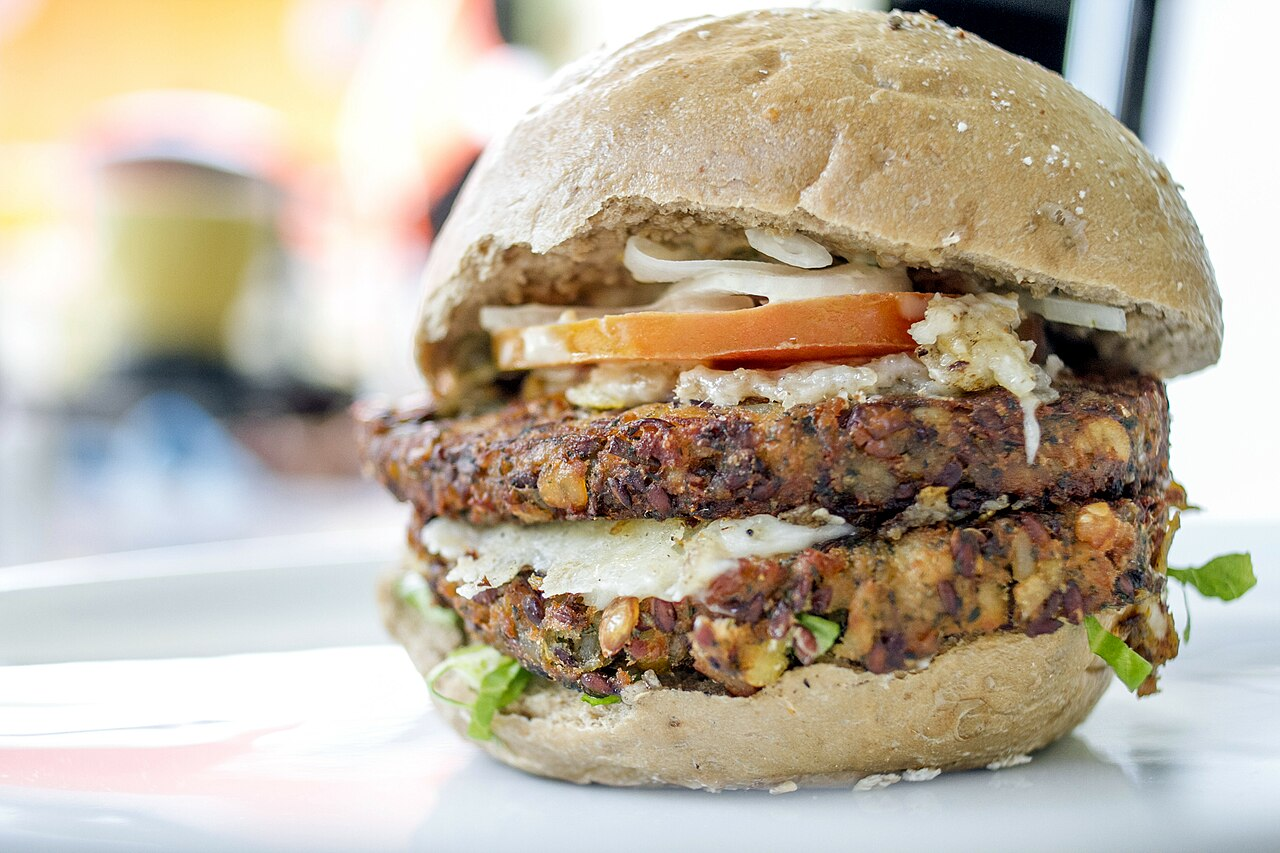
\includegraphics[width=0.7\textwidth]{images/burger.jpg}

By Roee Shpernik, CC BY-SA 4.0, https://commons.wikimedia.org/w/index.php?curid=35019440

\end{frame}


\begin{frame}
\frametitle{Burgers}

\centering
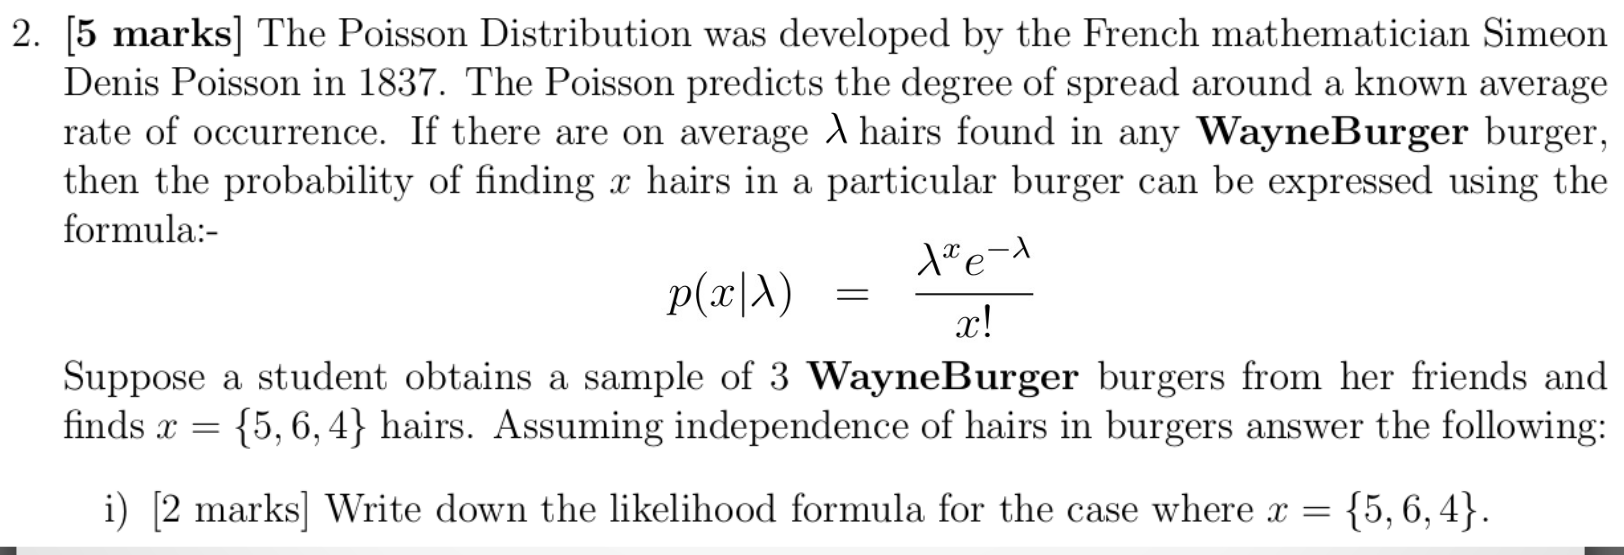
\includegraphics[width=0.7\textwidth]{images/wayneburger.png}

\end{frame}


\begin{frame}
\frametitle{Likelihood}
The likelihood function is formed from the product of the Poisson distribution
three times. Why? It's the probability of getting 5 hairs on the first burger
{\bf and} 6 on the second burger {\bf and} 4 on the third burger --- this is
the product rule in action.\pause
\begin{align}
p(x_1, x_2, x_3 \given \lambda)
    &= \frac{\lambda^{x_1}e^{-\lambda}}{x_1!}
        \frac{\lambda^{x_2}e^{-\lambda}}{x_2!}
        \frac{\lambda^{x_3}e^{-\lambda}}{x_3!} \\
    &\propto 
        \lambda^{x_1+x_2+x_3}e^{-3\lambda} \\
    &= \lambda^{15}e^{-3\lambda}.
\end{align}

\end{frame}


\begin{frame}
\frametitle{Log-Uniform Prior}
The log-uniform prior works nicely here because $\lambda$ must be positive,
and we can imagine being uncertain about the order of magnitude.\pause
\begin{align}
p(\lambda \given x_1, x_2, x_3) &\propto p(\lambda)p(x_1, x_2, x_3 \given \lambda) \\
    &\propto \frac{1}{\lambda} \lambda^{15}e^{-3\lambda} \\
    &= \lambda^{14}e^{-3\lambda}.
\end{align}
\pause
What distribution is this?

\end{frame}


\begin{frame}
\frametitle{Gamma Distribution}
Gamma distributions are used for positive quantities, and the
probability density function looks like this, with a polynomial factor
and an exponential factor:
\begin{align}
p(x \given \alpha, \beta)
    &= \frac{\beta^{\alpha}}{\Gamma(\alpha)}
            x^{\alpha-1}e^{-\beta x}.
\end{align}
\pause
As before, we can just focus on the part that depends on $x$ (which corresponds
to $\lambda$ on the previous slide). By matching terms we see that we have
\begin{align}
\lambda \given x_1, x_2, x_3 \sim \textnormal{Gamma}(15, 3).
\end{align}

\end{frame}


\begin{frame}
\frametitle{Our Gamma(15, 3) Posterior}

\centering
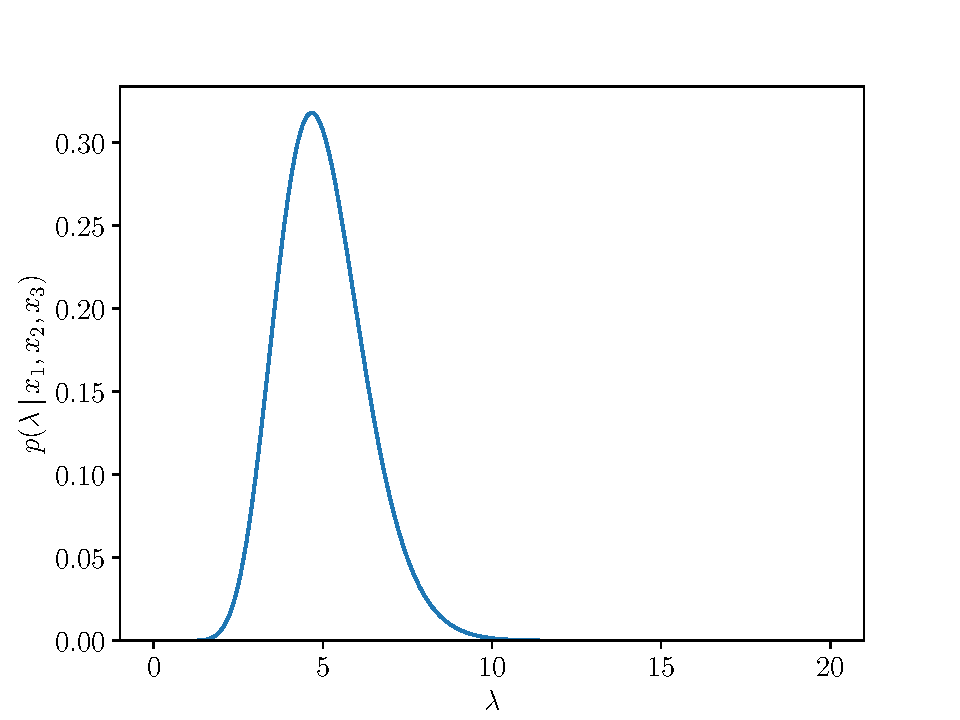
\includegraphics[width=0.6\textwidth]{images/gamma_posterior.pdf}

\end{frame}


\begin{frame}
\frametitle{Gamma Distributions from Wikipedia}
\centering
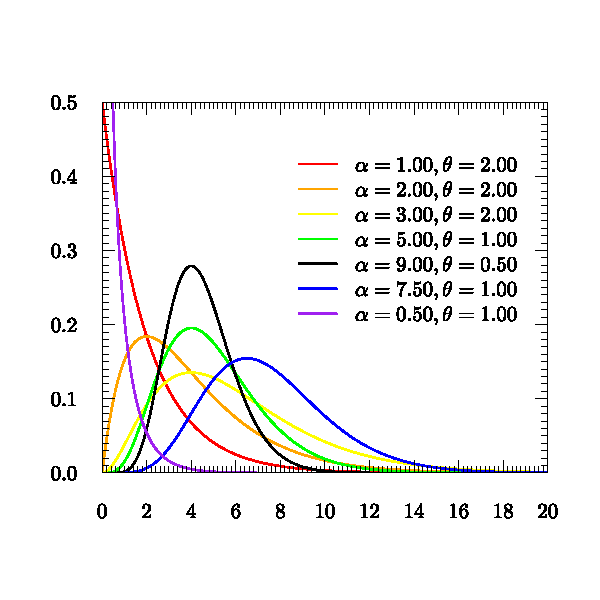
\includegraphics[width=0.7\textwidth]{images/gammas.pdf}

\end{frame}


\begin{frame}
\frametitle{Gamma-Poisson}

The gamma distribution is actually the conjugate prior for the Poisson distribution. This means:

Gamma Prior + Poisson Sampling Distribution $\implies$~Gamma Posterior.

Let's derive this now.


\end{frame}


\begin{frame}
\frametitle{Gamma-Poisson}
Suppose we have $x_1, x_2, ..., x_N$ and our sampling distribution for these
is Poisson with parameter/mean $\lambda$. We use a gamma prior for $\lambda$.
\pause
\begin{align}
p(\lambda \given x_1, ..., x_N)
    &\propto p(\lambda)p(x_1, ..., x_N \given \lambda) \\
    &\propto \lambda^{\alpha-1}e^{-\beta \lambda}
            \prod_{i=1}^N \lambda^{x_i}e^{-\lambda} \\
    &= \lambda^{\alpha - 1 + \sum_{i=1}^N x_i}e^{-(\beta + N)\lambda}
\end{align}
Therefore, the posterior is
\begin{align}
\lambda \given x_1, ..., x_N &\sim
    \textnormal{Gamma}\left(\alpha + \sum_{i=1}^N x_i, \beta + N\right).
\end{align}



\end{frame}


\begin{frame}
\frametitle{Gamma Distribution Summaries}
For a Gamma$(\alpha, \beta)$ distribution, the mean, variance, and mode
are given by
\begin{align}
\textnormal{mean} &= \frac{\alpha}{\beta} \\
\textnormal{variance} &= \frac{\alpha}{\beta^2} \\
\textnormal{mode} &= \left\{
                        \begin{array}{lr}
                        \frac{\alpha-1}{\beta},& \alpha \geq 1 \\
                        0,& \alpha < 1
                        \end{array}
                    \right.
\end{align}
\pause
If the gamma distribution is a conjugate prior, you can use these to summarise
both the prior and the posterior.


\end{frame}


\begin{frame}
\frametitle{Gamma as Conjugate Prior}
The gamma distribution is also the conjugate prior if the sampling
distribution is {\bf exponential}. Exponential distributions have a
`rate parameter' $\lambda$ and a probability density given by
\begin{align}
p(x \given \lambda) &= \lambda e^{-\lambda x}
\end{align}
where $x > 0$.

\end{frame}

\begin{frame}
\frametitle{Normal-Normal}
\begin{itemize}
\item The other famous conjugate prior is the normal-normal. However, this is a bit
messy, so I prefer to skip it in STATS 331 (it is studied in STATS 731).\pause
\item It also assumes the $\sigma$ of the normal distribution is known, which
is unrealistic.\pause
\item If you assume $\sigma$ is unknown, you can derive a posterior distribution
which is a Student-$t$ distribution.
\end{itemize}

\end{frame}


\begin{frame}
\frametitle{Uniform-Normal}
The normal-normal situation is too messy to cover here, but a simplified version
of it is worth knowing. Suppose the sampling distribution for the data is
a normal/gaussian distribution:
\begin{align}
x_1, ..., x_N \given \mu &\sim \textnormal{Normal}(\mu, \sigma^2)
\end{align}
\pause
We will assume that $\sigma$ is known (unrealistic) but $\mu$ is unknown.\pause

The PDF for the normal distribution is
\begin{align}
p(x \given \mu) &= \frac{1}{\sigma\sqrt{2\pi}}e^{-\frac{1}{2\sigma^2}(x-\mu)^2}.
\end{align}

\end{frame}


\begin{frame}
\frametitle{Uniform-Normal}
Let's assume a uniform prior for $\mu$.
Bayes' rule will give us the posterior:
\begin{align}
p(\mu \given x_1, ..., x_N) &\propto p(\mu)p(x_1, ..., x_N \given \mu) \\
    &\propto 1 \times \prod_{i=1}^N e^{-\frac{1}{2\sigma^2}(x_i - \mu)^2}
\end{align}
(I have ignored the normalising constant because it doesn't depend on $\mu$).

\end{frame}

\begin{frame}
\frametitle{Uniform-Normal}
We can take the product inside the exponential, where it becomes a sum:
\begin{align}
p(\mu \given x_1, ..., x_N) &\propto
    e^{-\frac{1}{2\sigma^2}\sum_{i=1}^N(x_i - \mu)^2}
\end{align}
\pause
After some steps, which I will skip, we can get the result and recognise it.
\begin{align}
\mu \given x_1, ..., x_N &\sim \textnormal{Normal}\left(\bar{x}, \frac{\sigma^2}{N}\right).
\end{align}
\pause
i.e., a normal distribution centered at the mean of the data, with a reduced
standard deviation.



\end{frame}



\begin{frame}
\frametitle{Analytical Methods: Pros and Cons}

{\bf Pros}
\begin{itemize}
\item Answers are exact with no need for approximate grids.\pause
\item The posterior distribution is often easy to use to compute
    predictions or summaries (we will look at summaries soon).
\end{itemize}
\pause
{\bf Cons}
\begin{itemize}
\item The trick of `recognising' the posterior distribution from its formula
is only possible in a few special cases.
\end{itemize}


\end{frame}



\begin{frame}
\frametitle{Analytical Marginalisation}
Suppose you obtain a joint posterior for two parameters $a$
and $b$, given some data $x$:
\begin{align}
p(a, b \given x) &\propto p(a, b)p(x \given a, b).
\end{align}
This would be a complicated formula involving $a$ and $b$.
\pause
To get the marginal distribution for $a$, you would do this integral
\begin{align}
p(a \given x) &= \int p(a, b \given x) \, db.
\end{align}
In many cases with conjugate priors this is possible analytically,
but we are not going to focus on it.



\end{frame}




\begin{frame}
\begin{center}
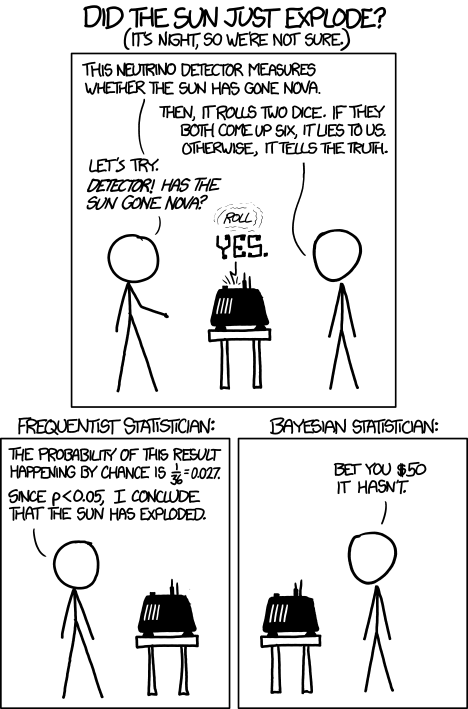
\includegraphics[width=0.4\textwidth]{images/xkcd.png} \\
Credit: Randall Monroe, xkcd
\end{center}

\end{frame}

\begin{frame}
\begin{center}
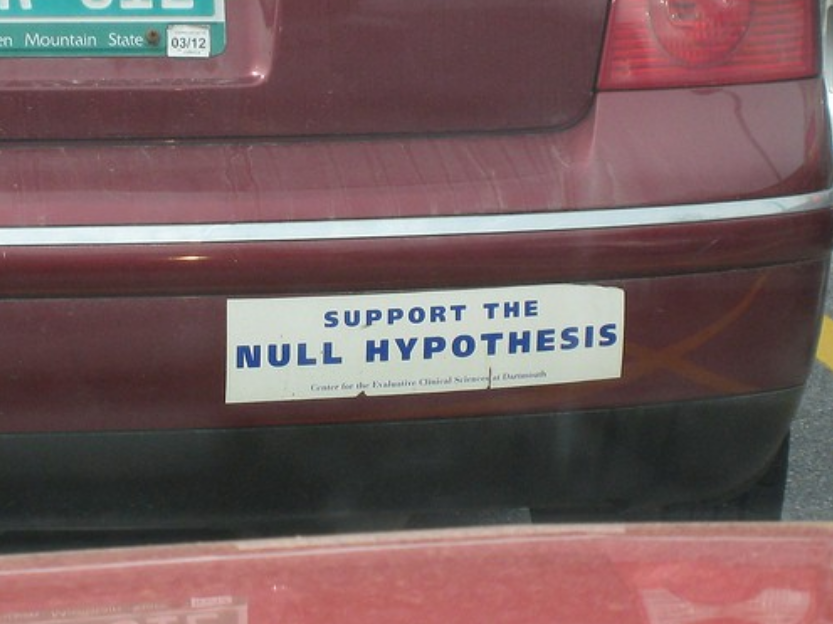
\includegraphics[width=0.6\textwidth]{images/support_null.png} \\
Credit: Unknown
\end{center}

\end{frame}

\begin{frame}
\begin{center}
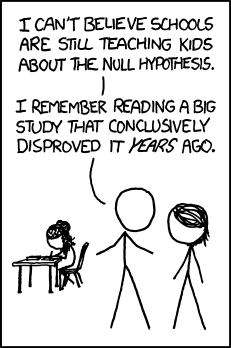
\includegraphics[width=0.4\textwidth]{images/null_hypothesis.png} \\
Credit: Randall Monroe, xkcd
\end{center}

\end{frame}


\begin{frame}
\frametitle{A Hypothesis Testing Scenario}
What if we considered these two hypotheses, as statisticians often do:
\begin{align}
H_0: \theta = 0.5 \\
H_1: \theta \neq 0.5
\end{align}
\pause

There might be a good reason to suspect the `null hypothesis' is true ---
e.g. if the effect being studied is absent.\pause

Classical/frequentist statistics would use {\bf p-values} for this, but we
will not.
\end{frame}


\begin{frame}
\frametitle{Hypothesis Testing vs. Parameter Estimation}
When we write down a list of hypotheses and get their
posterior probabilities (e.g., in a Bayes Box), we have tested all of the
hypotheses using the data. So there is not much else to do.
\pause
\begin{itemize}
\item In classical statistics, estimation and hypothesis testing
are quite distinct and are approached using different techniques.\pause
\item For us, they're basically the same thing --- except sometimes we will use a
different prior.
\end{itemize}

\end{frame}


\begin{frame}
\frametitle{Ed Jaynes Quote}

    \begin{columns} % Create two columns
        \column{0.5\textwidth} % Left column (50% width)
        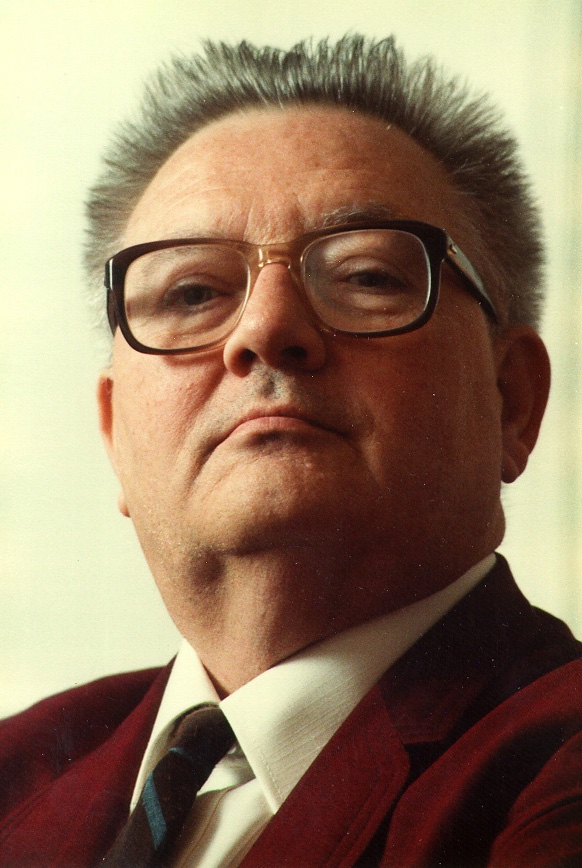
\includegraphics[width=0.7\linewidth]{images/jaynes.jpg}

        \column{0.5\textwidth} % Right column (50% width)
        {\em ``Any hypothesis testing
procedure can be
replaced by a parameter
estimation procedure that
is simpler and more
informative.''}
     \end{columns}

\end{frame}


\begin{frame}
\frametitle{Bus Problem}
When I first moved to Auckland, I caught buses arbitrarily, hoping I would
get to the right place. I achieved $x=2$ successes out of $N=5$ trials.
The binomial sampling distribution applies to $x$ here.\pause

Suppose we wanted to test $H_0: \theta = 0.5$. The p-value would be
\begin{align}
\textnormal{p-value} &= P(x \leq 2 \vee x \geq 3 \given H_0) = 1.
\end{align}
\pause
Traditionally, a statistician would say there is no evidence against the null
hypothesis. But is there evidence {\em for} it? In the Bayesian version of
hypothesis testing, we will be able to say that sometimes.

\end{frame}

\begin{frame}
\frametitle{Criticisms of P-Values}
Many people have criticised p-values. Some of the arguments include, but are not
limited to:
\begin{itemize}
\item P-values are not the probability of the null hypothesis, but are sometimes
interpreted as if they were.\pause
\item Frequentist statisticians know they are not. However, they are obviously
an attempt to quantify the plausibility of $H_0$.\pause
\item They do not take into account what you would have expected to observe if
$H_0$ were false.\pause
\item They are based on the probability of data that did not occur
(hypotheses in the tails).
\end{itemize}

\end{frame}

\begin{frame}
\frametitle{Harold Jeffreys Quote}

    \begin{columns} % Create two columns
        \column{0.5\textwidth} % Left column (50% width)
        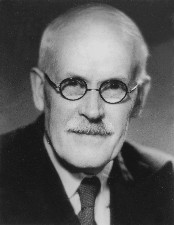
\includegraphics[width=0.7\linewidth]{images/jeffreys.jpg}

        \column{0.5\textwidth} % Right column (50% width)
        {\em ``A hypothesis may be rejected because it has not predicted
               observable results that did not occur!''}
     \end{columns}

\end{frame}

\begin{frame}
\frametitle{Spike and Slab Prior}
For us, the only distinction between a hypothesis testing situation and a
parameter estimation one is that a particular value of the parameter has
been singled out for special attention --- usually because it's plausible.\pause

To take this into account, all we have to do is give the special value of
$\theta$ more prior probability than it would have otherwise. This leads
to a `spike' in the prior. The rest of the $\theta$ values form a `slab'.
\end{frame}


\begin{frame}
\frametitle{Bayes Box: Uniform Prior}

\centering
{\footnotesize
\begin{tabular}{|c|c|c|c|c|}
\hline
Parameter & Prior & Likelihood & Prior $\times$ Likelihood & Posterior \\
$\theta$  & $p(\theta)$ & $p(x \given \theta)$ & $p(\theta)p(x\given \theta)$ & $p(\theta\given x)$ \\
\hline
0 & 0.0909 &  & & \\
0.1 & 0.0909  &   & & \\
0.2 & 0.0909 &  &  &  \\
0.3 & 0.0909 &  &  &  \\
0.4 & 0.0909 &  &  &  \\
0.5 & 0.0909 &  &  &  \\
0.6 & 0.0909 &  &  &  \\
0.7 & 0.0909 &  &  &  \\
0.8 & 0.0909 &  &  &  \\
0.9 & 0.0909 &  &  &  \\
1 & 0.0909 &  &  &  \\
\hline
Total & 1 & & & 1 \\
\hline
\end{tabular}
}

\end{frame}

\begin{frame}
\frametitle{Bayes Box: Spike and Slab Prior}

\centering
{\footnotesize
\begin{tabular}{|c|c|c|c|c|}
\hline
Parameter & Prior & Likelihood & Prior $\times$ Likelihood & Posterior \\
$\theta$  & $p(\theta)$ & $p(x \given \theta)$ & $p(\theta)p(x\given \theta)$ & $p(\theta\given x)$ \\
\hline
0 & 0.05 & 0 & 0 & 0\\
0.1 & 0.05 & 0.0729  & 0.003645 & 0.0163\\
0.2 & 0.05 & 0.2048 & 0.01024  & 0.0457 \\
0.3 & 0.05 & 0.3087 & 0.01544 & 0.0689 \\
0.4 & 0.05 & 0.3456 & 0.01728 & 0.0772 \\
{\bf 0.5} & {\bf 0.5} & {\bf 0.3125} & {\bf 0.1563} & {\bf 0.6977} \\
0.6 & 0.05 & 0.2304 & 0.0115 & 0.0514 \\
0.7 & 0.05 & 0.1323 & 0.0662 & 0.0295 \\
0.8 & 0.05 & 0.0512 & 0.00256 & 0.0114 \\
0.9 & 0.05 & 0.0081 & 0.000405 & 0.0018 \\
1 & 0.05 & 0 & 0 & 0 \\
\hline
Total & 1 & & 0.224 & 1 \\
\hline
\end{tabular}
}

\end{frame}

\begin{frame}[fragile]
\frametitle{Constructing the Spike and Slab Prior in R}
You first create the slab, then manually put in the spike.

\begin{minted}{r}
theta = seq(0, 1, by=0.1)
prior = rep(0.5/(length(theta)-1), length(theta))
prior[abs(theta - 0.5) < 1E-7] = 0.5
\end{minted}
\pause

{\bf Note}: Instead of testing for exact equality of the
\mintinline{r}{theta} values to 0.5, I just found the
value close to 0.5. This is more robust due to computer weirdness.
\end{frame}

\begin{frame}[fragile]
\frametitle{Bus Problem Likelihood}
For completeness, here is the likelihood for the bus problem.

\begin{minted}{r}
lik = dbinom(2, size=5, prob=theta)
\end{minted}
\end{frame}


\begin{frame}[fragile]
\frametitle{Key Differences from Frequentist Hypothesis Testing}

\begin{itemize}
\item No p-value. Instead, calculate the posterior probability of the null
hypothesis.\pause
\item This has a clearer interpretation, and is what we really want to know.\pause
\item You can get evidence {\bf for} the null hypothesis, if the data
suggests this. This happened in the bus example we just saw, as the
probability went up from 0.5 to 0.6977.
\end{itemize}

\end{frame}


\begin{frame}[fragile]
\frametitle{Terminology}
In Bayesian hypothesis testing (closely related to `Bayesian model selection'),
there is some additional terminology, and additional quantities that people
like to talk about.\\[0.5em]

Some of these are the {\bf evidence (marginal likelihood)},
the {\bf Bayes factor}, and the {\bf odds ratio}.\\[0.5em]

These re-express the same conclusions that we already have with posterior
probabilities, but in a different form.

\end{frame}


\begin{frame}
\frametitle{Bayes' Rule Twice}
Here is Bayes' rule twice, expressing the posterior probabilities of two
hypotheses $H_0$ and $H_1$:
\begin{align}
P(H_0 \given x) &= \frac{P(H_0)p(x \given H_0)}{p(x)} \\
P(H_1 \given x) &= \frac{P(H_1)p(x \given H_1)}{p(x)}
\end{align}
\pause

{\bf Note}: I have written upper case $P$ for the terms that are
definitely probabilities, and lower case for the ones that might
be probabilities or probability densities.


\end{frame}


\begin{frame}
\frametitle{Division}
If we divide the two equations by each other, the denominators cancel out,
leaving us with ``Bayes' rule in odds form'':
\begin{align}
\frac{P(H_0 \given x)}{P(H_1 \given x)}
    &= \frac{P(H_0)}{P(H_1)} \times \frac{p(x \given H_0)}{p(x \given H_1)}.
\end{align}
\pause
or
\begin{align}
\textnormal{posterior odds} &=
    \textnormal{prior odds} \times \textnormal{Bayes factor}.
\end{align}


\end{frame}


\begin{frame}
\frametitle{Bus Result Expressed Differently}
\begin{itemize}
\item In the bus problem, the prior probability of $H_0$ was 0.5, so the prior
odds ratio was $0.5/(1 - 0.5) = 1$. The posterior probability was
0.6977 so the posterior odds ratio was $0.6977/(1 - 0.6977)=2.308$.\pause
\item That is, the data makes $H_0$ 2.308 times more probable than $H_1$.\pause
\item We can also solve for the Bayes factor, which must equal the posterior
odds ratio because the prior odds ratio was 1. Therefore the Bayes factor
is also 2.308 --- the data was 2.308 times more probable under $H_0$ than
under $H_1$.
\end{itemize}


\end{frame}


\begin{frame}
\frametitle{MacKay Biased Coin Example}

\begin{center}
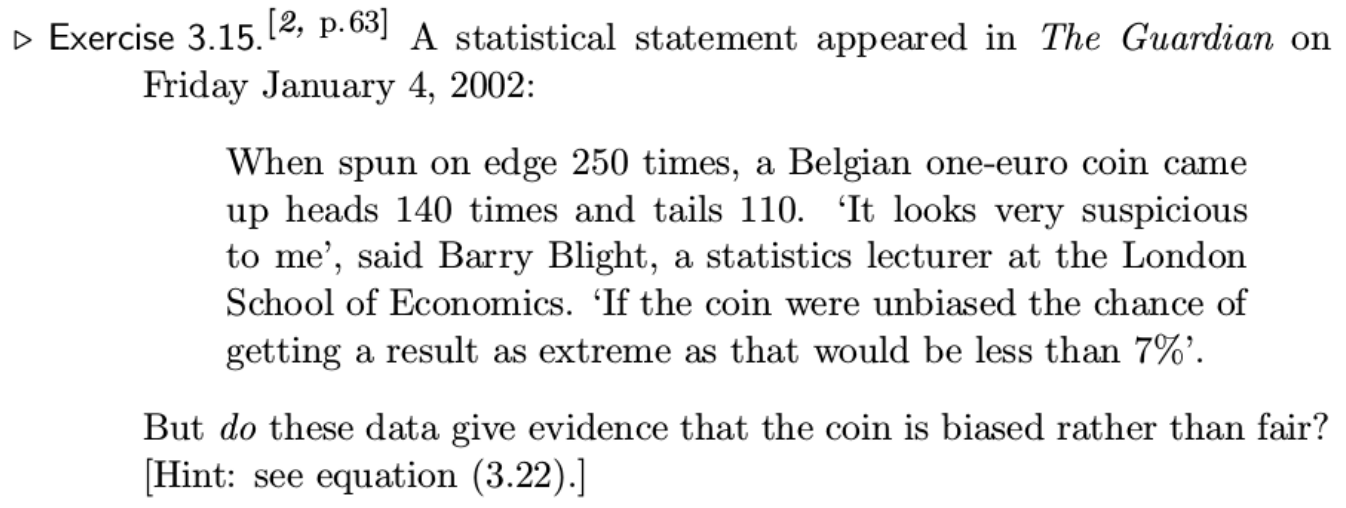
\includegraphics[width=0.9\textwidth]{images/mackay_coin.png}
\end{center}

Let's do this with a spike and slab prior.

\end{frame}

\begin{frame}
\frametitle{MacKay Biased Coin Example}

\centering
Computational Interlude

\end{frame}



\begin{frame}
\frametitle{MacKay Biased Coin Example: Second Method}
There is another way to do this calculation, which is actually more common
and more general than using a spike and slab prior. Look at Bayes' rule
in odds form again:
\begin{align}
\frac{P(H_0 \given x)}{P(H_1 \given x)}
    &= \frac{P(H_0)}{P(H_1)} \times \frac{p(x \given H_0)}{p(x \given H_1)}.
\end{align}
\pause

If we can calculate the numerator and denominator in the Bayes factor part,
we can get the Bayes factor and the posterior odds, i.e., the conclusion.
\end{frame}

\begin{frame}
\frametitle{Bayesian Model Comparison}
Consider two `models' $M_1$ and $M_2$ with unknown parameters $\theta_1$
and $\theta_2$ respectively. To get the Bayes factor we would need likelihood
values $P(x \given M_1)$ and $P(x \given M_2)$.\\[0.5em]\pause

When we do parameter estimation within $M_1$, we get the marginal likelihood
\begin{align}
p(x \given M_1) &= \sum_{\theta_1} p(\theta_1 \given M_1)p(x \given \theta_1, M_1)
\end{align}

This, and the corresponding value for $M_2$, is just what we need for the Bayes factor!

\end{frame}

\begin{frame}
\frametitle{Evidence}

That's why marginal likelihood
is sometimes called evidence --- that number indicates how strongly the data supports
{\em any} of the $\theta$ values --- i.e., your whole underlying model.

\end{frame}


\begin{frame}[fragile]
\frametitle{MacKay Coin Example: The Numerator}
Since $H_0$ asserts a single value for $\theta=0.5$, the term in the numerator
of the Bayes factor is really just the likelihood for $\theta=0.5$:
\begin{minted}{r}
lik_H0 = dbinom(140, size=250, prob=0.5)
\end{minted}
\pause

$H_1$ is more complex, because it involves multiple values of $\theta$.
However, as we just saw, we need the marginal likelihood from estimating $\theta$ assuming $H_1$.
\end{frame}

\begin{frame}[fragile]
\frametitle{MacKay Coin Example: The Denominator}
This looks just like parameter estimation, except for the Bayes factor
calculation at the end.
\begin{minted}{r}
theta = seq(0, 1, by=0.001)
prior = rep(1/length(theta), length(theta))
lik = dbinom(140, size=250, prob=theta)
h = prior*lik
Z = sum(h) # This is what we need
bayes_factor = lik_H0/Z
\end{minted}
\pause
The result is approximately 2.1, so we have evidence in favour of
$H_0$.

\end{frame}

\begin{frame}[fragile]
\frametitle{Converting Back to Posterior Probabilities}
If we have the conclusion in terms of posterior probabilities, it is easy
to get the posterior odds or Bayes factor, as we saw with the bus example.
How do we do the reverse? Make a tiny Bayes Box!

\end{frame}

\begin{frame}[fragile]
\frametitle{Tiny Bayes Box}

\begin{minted}{r}
> prior2 = c(0.5, 0.5)
> lik2 = c(lik_H0, Z)
> h2 = prior2*lik2
> Z2 = sum(h2)
> post2 = h2/Z2
> post2
[1] 0.6773934 0.3226066
\end{minted}


\end{frame}

\begin{frame}
\frametitle{Warning}

\begin{itemize}
\item Bayesian model selection results
can depend strongly on priors, such as the width/shape of the slab. You usually
can't get away with naive choices like super-wide uniform distributions.\pause
\item Why? The priors change what data you would expect to observe under each
hypothesis/model.\pause
\item E. T. Jaynes quote:
\end{itemize}

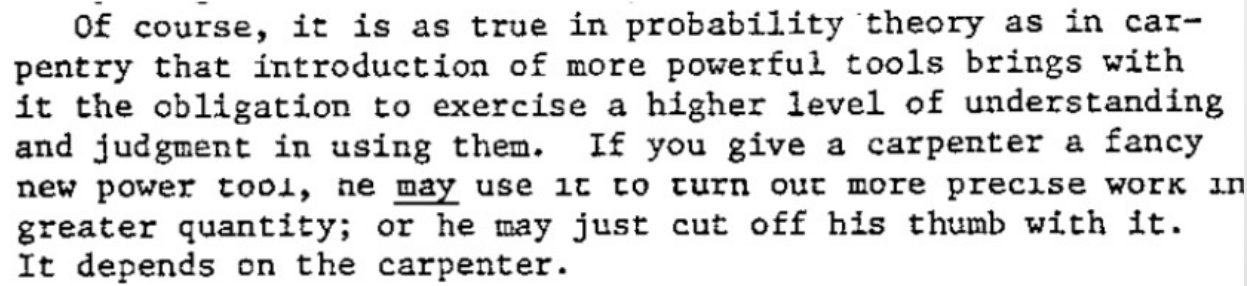
\includegraphics[width=0.8\textwidth]{images/carpenter.png}

\end{frame}




\end{document}

